\section*{Problem Sheet 3:}
\label{sec:ps3}
\newcounter{psThreeQuestions}
\setcounter{psThreeQuestions}{0}
\renewcommand{\NewQuestion}[1]{\stepcounter{psThreeQuestions}\subsection*{Exercise \arabic{psThreeQuestions}: #1}}


\NewQuestion{CP-violating interference effects in \prt{B^{-} \to DK^{-}}}
This question looks ahead to the topics covered in weeks 4/5. So do not panic if you do not recognise it from the lectures - this is because we haven't done this, yet. The idea is a "guided exploration" of something new. Educational scientists tell me that this is a very good way to learn.
If you stick with it until the end, the question also introduces you to a decay where you see huge CP violation effects.

\begin{enumerate}[a)]
\item Consider the decays \prt{B^- \to D^0 K^-} and \prt{B^- \to \overline{D}^0 K^-}. 
 \begin{itemize}
 \item Use the formula sheet to find out the quark content of the mesons involved.
 \answerbox{
 $\prt{B^-} = (b, \overline{u})$, \\
 $\prt{D^0} = (c, \overline{u})$ (and hence $\prt{\overline{D^0}} = (\overline{c}, u)$,\\
 $\prt{K^-} = (s, \overline{u})$.
 }
 \item Draw the tree-level Feynman diagrams that describe these decays. There are two topologies, they look like this:\\
 \begin{tabular}{cc}
 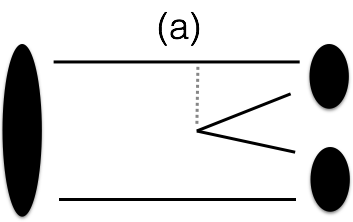
\includegraphics[width=0.3\textwidth]{problemsheets/ps2figs/CSup} &
 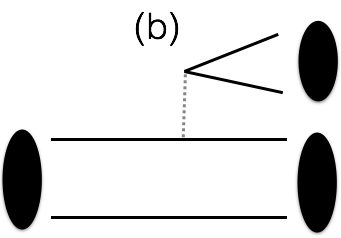
\includegraphics[width=0.3\textwidth]{problemsheets/ps2figs/CFav}
 \end{tabular}\\
 where the black blobs indicate that two quarks form a meson.
 \answerbox{The diagrams look like this:\\
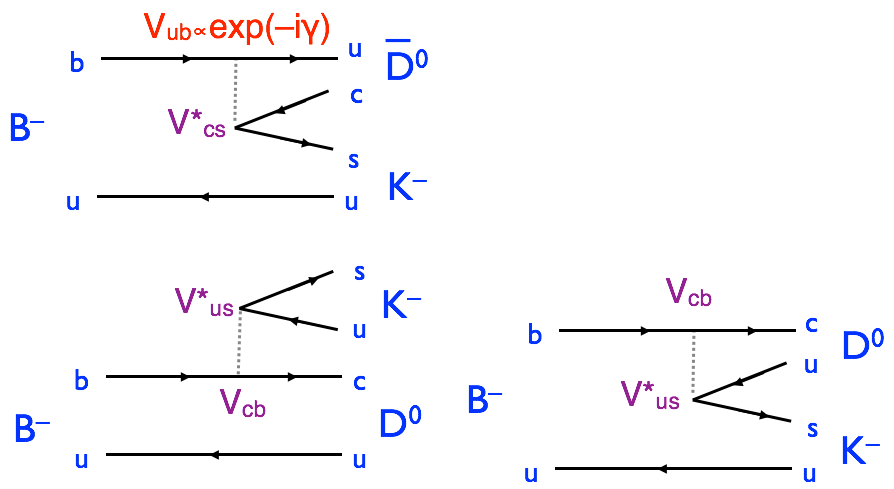
\includegraphics[width=0.7\textwidth]{problemsheets/ps2figs/B2DKDiagrams.png}
}
 \item One of the topologies for the \prt{B^-} decay diagrams given above is "colour-suppressed". This means that the requirement that mesons are colourless objects restricts the colours that the quarks that result from this decay can have (while for the other diagram there is no such restriction). Which topology is colour suppressed? Explain, why.
 \answerbox{ (Remember, quarks can be red, green, blue, anti-quarks can
  be anti-red, anti-green, anti-blue; colourless objects can be made
  by combining three quarks: red + green + blue = white; or three
  anti-quarks: anti-red, plus anti-green plus anti-blue is also white;
  or by combining quark-antiquark pairs like red + anti-red, or green
  + anti-green, or blue + anti-blue.)
  \vspace{2ex}\\
  Topology (a) is colour suppressed. This is because in this diagram:
  \\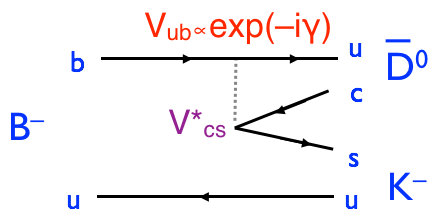
\includegraphics[width=0.5\textwidth]{problemsheets/ps2figs/B2DK_supp}\\
  the \prt{B^-} is colour neutral, so it is a colour - anti-colour
  pair (say red and anti-red). The $\overline{c}$ and $s$ quark must
  then have the same anti-colour/colour as the $\overline{b}$ and $u$
  quark we started off with, in order to produce colour-less mesons
  (in our example anti-red, red). The \prt{B^-} is colourless, so if,
  for example, the $b$ is red, than the $\overline{u}$ must be anti-red }
 \item One of the two decays can proceed via both topologies (colour favoured and colour suppressed), the other only by one of them. To simplify the rest of the question a bit: for the decay where both topologies apply, only consider the colour favoured diagram and ignore the suppressed.
 \answerbox{... so this means that you should only consider these two diagrams:
 \\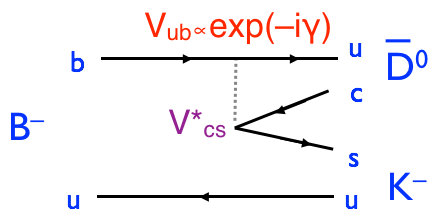
\includegraphics[width=0.5\textwidth]{problemsheets/ps2figs/B2DK_supp}, 
 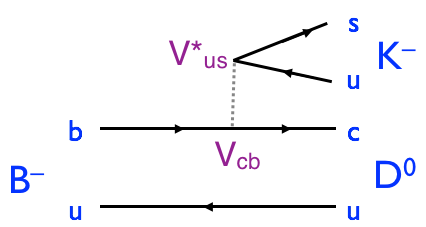
\includegraphics[width=0.5\textwidth]{problemsheets/ps2figs/B2DK_fav}.
 }
 \item Estimate the complex value of the ratio of the two diagrams
  \[
    r_B e^{i\phi} = \frac{A(\prt{B^- \to \Dob K^-})}{\prt{A(B^- \to \Do K^-})}
 \]
 expressed as a magnitude $r_B$ and phase $\phi$. You obtain this value
 by multiplying together the vertex factors and multiplying the colour-suppressed diagram by $1/\sqrt{3}$ to take into account the colour suppression. {\bf Hint:} For two generations of quarks, you know how to do the vertices - the vertex factors are $g_{W}$ multiplied by $\cos{\theta_C}$ or $\pm \sin\theta_C$. For three generations of quarks (we have a $b$ meson involved), you need to use the CKM matrix elements given in the formula sheet instead. These are applied like this:
 \\
 \begin{tabular}{cc}
 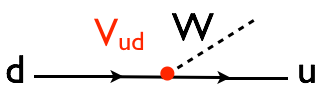
\includegraphics[width=0.3\textwidth]{problemsheets/ps2figs/CKM_Vud}
 &
 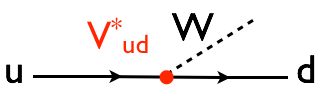
\includegraphics[width=0.3\textwidth]{problemsheets/ps2figs/CKM_Vudstar}
\end{tabular}\\
 Where you can replace $u$ with any up-type quark ($u, c, t$) and $d$ with any down-type quark ($d, s, b$), for example:
 \\
 \begin{tabular}{cc}
 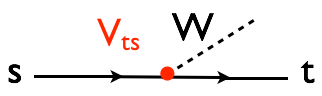
\includegraphics[width=0.3\textwidth]{problemsheets/ps2figs/CKM_Vts}
 &
 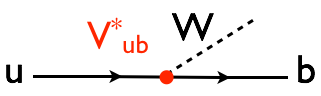
\includegraphics[width=0.3\textwidth]{problemsheets/ps2figs/CKM_Vubstar}
 \end{tabular}\\
 Note the complex conjugation if you go from up-type to down-type, which matters for the complex CKM elements $V_{ub}$ and $V_{td}$. You can rotate these vertices around as you like, for example:
 \\
 \begin{tabular}{cccc}
 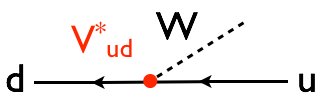
\includegraphics[width=0.25\textwidth]{problemsheets/ps2figs/CKM_Vudstar_anti}
 &
 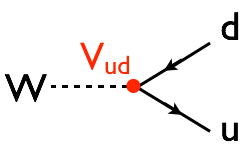
\includegraphics[width=0.2\textwidth]{problemsheets/ps2figs/CKM_Vud_create}
 &
 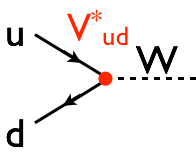
\includegraphics[width=0.15\textwidth]{problemsheets/ps2figs/CKM_Vudstar_annihilate}
 &
 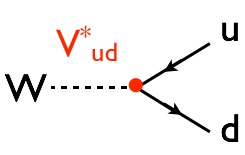
\includegraphics[width=0.2\textwidth]{problemsheets/ps2figs/CKM_Vudstar_create}
 \end{tabular}
 \end{itemize}  
 \answerbox{
    The value of the \prt{\Bm \to \Dob \Km} diagram (i.e. the product of the relevant vertex factors) is $g_W V_{ub} \cdot g_W V^*_{cs}$. For \prt{\Bm \to \Dob \Km} it is $g_W V_{cb} \cdot g_W V_{us}^*$. The colour suppression introduces an additional factor of $1/\sqrt{3}$ to the \prt{\Bm \to \Dob \Km} diagram. So the ratio is:
    \[
    r_B e^{i\phi}  = \frac{A(\prt{B^- \to \Dob K^-})}{\prt{A(B^- \to \Do K^-})} = 
    \frac{V_{ub} \cdot V^*_{cs}}{\sqrt{3} \; V_{cb} \cdot V_{us}^*}
    \]
    From the formula sheet: 
    \begin{itemize}
     \item $V_{ub}   = 0.0037 \cdot e^{-i\gamma}$
     \item $V_{cs}^* = 0.97$
     \item $V_{cb}   = 0.041$
     \item $V_{us}^* = 0.23$
    \end{itemize}
    With this I get: $r_B e^{i\phi} = 0.22 e^{-i\gamma} = 0.22 e^{-i (68^{\circ})}$
 }
%%
\item Now consider the decay chains
\prt{B^- \to D^0 K^-, \Do \to K^+ K^-} and \prt{B^- \to \overline{D}^0 K^-, \Dob \to K^+ K^-}.
 \begin{itemize}
 \item Note that these two decay paths will interfere with each other - the situation is analogous to the double slit experiment:
 \\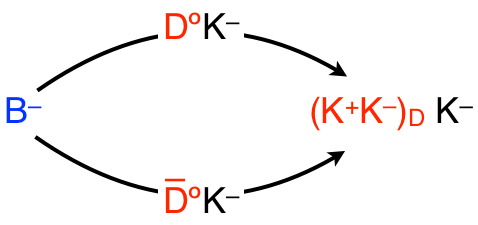
\includegraphics[width=0.5\textwidth]{problemsheets/ps2figs/B2DK_D2KK_interference}
 \item A bit of notation: To refer to the full decay that includes the interference between these decay paths, we write
 \prt{B^- \to (K^+ K^-)_D K^-}.
 Here, the notation \prt{(K^+K^-)_D} simply indicates that the \prt{K^+} and \prt{K^-} result from the decay of the \Do\ or \Dob. 
 \item Interference leads to sensitivity to phases - specifically, to sensitivity to the phase difference between the two decay paths. Your Feynman diagrams should indicate a phase difference of $\phi = -\gamma$ due to the weak interaction. This, however, neglects the effects of the strong interaction. This is difficult to calculate but it also leads to a phase difference, which we call $\delta_B$. So the total phase difference is $\phi = \delta_B - \gamma$.
 \item For the next step, it's useful to define:
 \begin{itemize}
 \item $C$ is the amplitude $A(\prt{B^- \to D^0 K^-})$.
 \item We write the amplitude ratio of \prt{B^- \to \Dob K^-} and \prt{B^- \to \Do K^-} as
 \[
    \frac{A(\prt{B^- \to \Dob K^-})}{\prt{A(B^- \to \Do K^-})} = r_B e^{i(\delta_B - \gamma)}
 \]  
 where $r_B$ is the magnitude of this ratio, $\delta_B$ the phase difference induced by the strong interaction, and $\gamma$ the CP violating one induced by the weak interaction.
 \item $K$ is the amplitude $A(\prt{ \Do \to K^+ K^-})$, which is the same as $A(\prt{ \Dob \to K^+ K^-})$ (you can check by drawing the diagrams and applying CKM factors).
 \end{itemize}
 With this, we can label our interference sketch with the relevant amplitudes like this:\\
 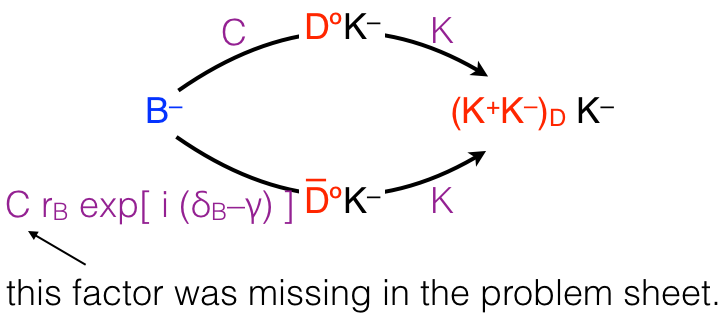
\includegraphics[width=0.5\textwidth]{problemsheets/ps2figs/B2DK_D2KK_interference_labelled}\\
 (This has no purpose other than visualising and organising what goes on, which can be helpful in the subsequent calculations.)
 \item If you apply the \cp\ operation to this amplitude ratio, you get:
  \[
    \frac{A(\prt{B^+ \to \Do K^+})}{\prt{A(B^+ \to \Dob K^+})} = r_B e^{i(\delta_B + \gamma)}
 \]
 Explain why.
 \answerbox{The strong interaction respects \cp\ symmetry, so all factors introduced by it (including the phase $\delta_B$) remain invariant. For the weak interaction, the \cp\ operation has the effect of complex conjugating the CKM matrix element, so we take the negative of all phases introduced by the CKM matrix, here: $\gamma \to -\gamma$. The magnitudes remain the same, so:
 $
 \left|\frac{A(\prt{B^- \to \Dob K^-})}{\prt{A(B^- \to \Do K^-})} \right| = 
 \left|\frac{A(\prt{B^+ \to \Do K^+})}{\prt{A(B^+ \to \Dob K^+})} \right|
 $
 and hence, the effect of \cp\ is: $r_B \to r_B$, $\delta_B \to \delta_B$, $\gamma \to -\gamma$.
 }
 \item Calculate the rate asymmetry
 \[
  A = \frac{ 
    \Gamma(B^- \to (K^+ K^-)_D K^-) -
    \Gamma(B^+ \to (K^+ K^-)_D K^+)
  }{ 
    \Gamma(B^- \to (K^+ K^-)_D K^-) +
    \Gamma(B^+ \to (K^+ K^-)_D K^+)
  }
 \]
 in terms of $r_B$, $\delta_B$, $\gamma$ (the $C$ and $K$ will cancel, if you want you can simply set them to $1$ straight from the beginning).
 \end{itemize}
 \answerbox{
     \begin{eqnarray*}
      \Gamma(B^-) & = & 
      \left| CK e^{i\delta_D^{K\pi}} + CK r_B e^{i(-\gamma + \delta_B)} \right|^2
      \\ & = &
      C^2 K^2 \left(1 + r_B^2 + 2\,r_B\,\cos\left(-\gamma +\delta_B \right)\right)
      \\ & = & C^2K^2\left(1 + r_B^2 + 2\,r_B\, \left(
        \cos(\delta_B)\,\cos\gamma {\color{red} +} 
        \sin(\delta_B)\,\sin\gamma\right)\right)
      \\ \Gamma(B^+) & = & 
      \left| CK + CK r_B e^{i(+\gamma + \delta_B)} \right|^2
      \\ & = &
      C^2 K^2 \left(1 + r_B^2 + 2 r_B\,\cos\left(+\gamma +\delta_B \right)\right)
      \\ & = & C^2 K^2 \left(1 + r_B^2 + 2 r_B\, \left(
        \cos(\delta_B)\,\cos\gamma {\color{red} -}
          \sin(\delta_B)\,\sin\gamma\right)\right)
      \\ A_{CP}^{KK} & = & 
      \frac{
        2 r_B\,\sin(\delta_B)\,\sin\gamma
      }{
        1 + r_B^2 + r_B\, \cos(\delta_B)\,\cos\gamma
      } 
    \end{eqnarray*}
 }
 \item Repeat the calculation for
  \[
  A = \frac{ 
    \Gamma(B^- \to (K^+ \pi^-)_D K^-) -
    \Gamma(B^+ \to (K^- \pi^+)_D K^+)
  }{ 
    \Gamma(B^- \to (K^+ \pi^-)_D K^-) +
    \Gamma(B^+ \to (K^- \pi^+)_D K^+)
  }
 \]
 Note that there will additional parameters because the ratio of the \Do, \Dob\ decay amplitudes does not cancel as in the case above, but instead:
  \[
    \frac{A(\prt{\Do \to K^+ \pi^-})}{A(\prt{\Dob\to K^+\pi^-})} = r_D^{K\pi} e^{i\delta_D}
 \]
 \answerbox{
    In the previous part, with used
    $\frac{A(\prt{\Do \to K^+ K-})}{A(\prt{\Dob\to K^+K-})}=1$, which is fundamentally because there is no \cp\ violation in \Do\ decays, and the final state is a \cp\ eigenstate. We could also have arrived at this result by drawing the Feynman diagrams for both decays, using the appropriate CKM matrix elements (and that the CKM matrix elements involved in \Do\ decays are all real is ultimately the reason that there is no \cpv\ in \Do\ decays).
     
    Now that the \Do, \Dob\ do not decay to a \cp\ eigenstate anymore we actually need to take into account that 
    \[
    \frac{A(\prt{\Do \to K^+ \pi^-})}{A(\prt{\Dob\to K^+\pi^-})} = r_D^{K\pi}  e^{i\delta_D}
    \]
    Note that there is no weak phase that would change under \cp. You can get this by drawing diagrams, or just remember that there is no \cpv\ in D meson decays. So $\delta_D$ is the strong phase difference between the \Do\ and \Dob\ decay amplitude to $\Kp\pim$.
    
    Our interference sketch looks now like this:
    \\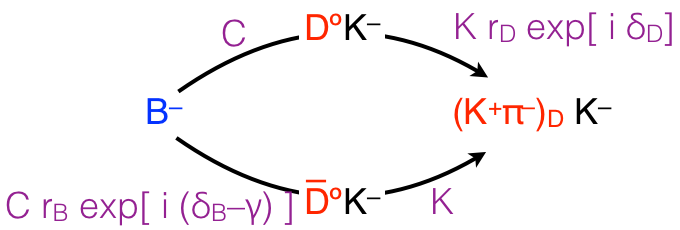
\includegraphics[width=0.5\textwidth]{problemsheets/ps2figs/B2DK_D2Kpi_Interference}\\
    
     \begin{eqnarray*}
      \Gamma(B^-) & = & 
      \left| CK r_D^{K\pi} e^{i\delta_D^{K\pi}} + CK r_B e^{i(-\gamma + \delta_B)} \right|^2
      \\ & = &
      C^2 K^2 \left({r_D^{K\pi}}^2 + r_B^2 + 2r_D^{K\pi}\,r_B\,\cos\left(-\gamma +\delta_B-\delta_D^{K\pi} \right)\right)
      \\ & = & C^2K^2\left({r_D^{K\pi}}^2 + r_B^2 + 2r_D^{K\pi}\,r_B\, \left(
        \cos(\delta_B-\delta_D^{K\pi})\,\cos\gamma {\color{red} +}
        \sin(\delta_B-\delta_D^{K\pi})\,\sin\gamma\right)\right)
      \\ \Gamma(B^+) & = & 
      \left| CK r_D^{K\pi} e^{i\delta_D^{K\pi}} + CK r_B e^{i(+\gamma + \delta_B)} \right|^2
      \\ & = &
      C^2 K^2 \left({r_D^{K\pi}}^2 + r_B^2 + 2r_D^{K\pi}\,r_B\,\cos\left(+\gamma +\delta_B-\delta_D^{K\pi} \right)\right)
      \\ & = & C^2 K^2 \left({r_D^{K\pi}}^2 + r_B^2 + 2r_D^{K\pi}\,r_B\, \left(
        \cos(\delta_B -\delta_D^{K\pi})\,\cos\gamma 
        {\color{red} -} \sin(\delta_B-\delta_D^{K\pi})\,\sin\gamma\right)\right)
      \\ A_{CP}^{K\pi} & = & 
      \frac{
        2r_D^{K\pi}\,r_B\,\sin(\delta_B-\delta_D^{K\pi})\,\sin\gamma
      }{
        {r_D^{K\pi}}^2 + r_B^2 + 2r_D^{K\pi}\,r_B\, \cos(\delta_B-\delta_D^{K\pi})\,\cos\gamma
      } 
      \\ & = & 
      \frac{
        2\,\frac{r_B}{r_D^{K\pi}}\,\sin(\delta_B-\delta_D^{K\pi})\,\sin\gamma
      }{
        1 + \left(\frac{r_B}{r_D^{K\pi}}\right)^2 
        + 2\frac{r_B}{r_D^{K\pi}} \cos(\delta_B-\delta_D^{K\pi})\,\cos\gamma
      } 
      \\ & & \mbox{which is the same as}
        \\ & = & 
      \frac{
        2\,\frac{r_D^{K\pi}}{r_B}\,\sin(\delta_B-\delta_D^{K\pi})\,\sin\gamma
      }{
        1 + \left(\frac{r_D^{K\pi}}{r_B}\right)^2 
        + 2\frac{r_D^{K\pi}}{r_B} \cos(\delta_B-\delta_D^{K\pi})\,\cos\gamma
      } 
    \end{eqnarray*}
 }
 \item Which of the two asymmetries is larger? Estimate an approximate numerical value.
 \answerbox{The difference between the two asymmetries is that, to get from $A_{CP}^{KK}$ to $A_{CP}^{K\pi}$,  we need to replace $r_B$ with $r_B/r_D^{K\pi}$, or, equivalently with $r_D^{K\pi}/r_B$. The best sensitivity is reached for when this factor is $\sim 1$, to the question comes down to whether $r_B$ or $r_D^{K\pi}/r_B$ is closer to $1$ (note
 
 So let's estimate $r_D$. The relevant Feynman diagrams are:
 \\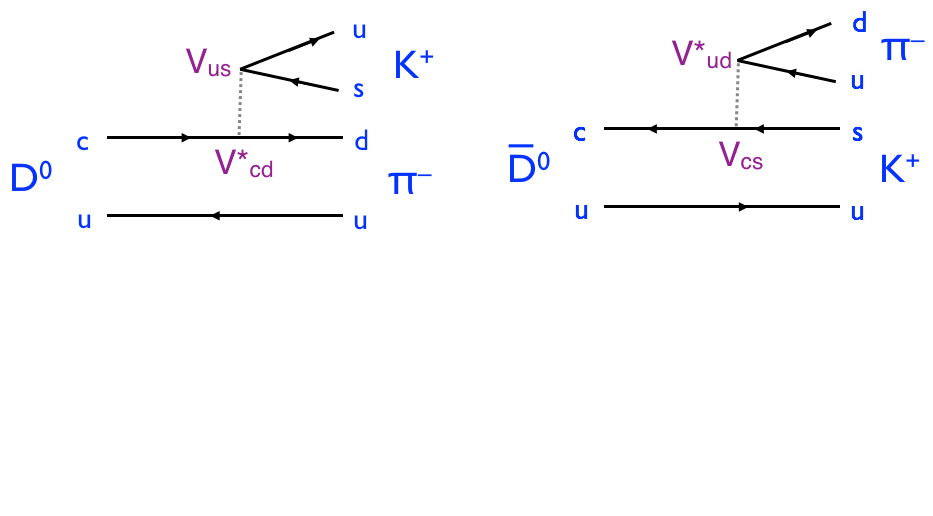
\includegraphics[width=0.65\textwidth]{problemsheets/ps2figs/D2KpiDiagrams}.\\
 Multiplying the relevant CKM matrix elements:
    \[
     \frac{A(\prt{\Do \to K^+ \pi^-})}{A(\prt{\Dob\to K^+\pi^-})}
     =
     \frac{V_{cd}^* V_{us}}{ V_{ud}^* V_{cs}}
     \approx \cos^2(\theta_C) = 0.05
    \]
 So, we estimate $r_D/r_B \sim 0.25$. It turns out that the measured values for $r_B$ is $0.01$, somewhat smaller than our estimate, while our estimate for $r_D$ is spot-on, so really, $r_D/r_B \sim 0.5$.
 
 To estimate the size of the asymmetry, we need to know $\delta_B$ and $\delta_D$. We cannot calculate those, but we can get an estimate of the maximum value that the asymetries can obtain by assuming they are such that the cosine of the strong phase differences is $0$ and the sine is $1$, leading to
 \begin{eqnarray*}
     A_{CP}^{KK} 
       & \leq & 
      \frac{
        2\,r_B\,\sin\gamma
      }{
        1 + r_B^2 
      }
  \\ A_{CP}^{K\pi} 
       & \leq & 
      \frac{
        2\,\frac{r_D^{K\pi}}{r_B}\,\sin\gamma
      }{
        1 + \left(\frac{r_D^{K\pi}}{r_B}\right)^2 
      } 
  \end{eqnarray*}
 Putting in the values we calculated in this exercise, we get
  \begin{eqnarray*}
     A_{CP}^{KK} 
       & \leq & 
      \frac{
        2 \cdot 0.22 \sin(68^{\circ})
      }{
        1 + 0.22^2 
      } = 0.38
  \\ A_{CP}^{K\pi} 
       & \leq & 
      \frac{
        2\cdot 0.25\,\sin(68^{\circ})
      }{
        1 + 0.25^2 
      } =0.48
  \end{eqnarray*}
 These are both quite large numbers (\cp\ assymetries of about 40-50\%, that's a big effect). Using the measured value of $r_B$ instead, we get
  \begin{eqnarray*}
     A_{CP}^{KK} 
       & \leq & 
      \frac{
        2 \cdot 0.1 \sin(68^{\circ})
      }{
        1 + 0.1^2 
      } = 0.18
  \\ A_{CP}^{K\pi} 
       & \leq & 
      \frac{
        2\cdot 0.5\,\sin(68^{\circ})
      }{
        1 + 0.5^2 
      } =0.74
  \end{eqnarray*}
 Now the difference between the two methods becomes much clearer. While $A_{CP}^{KK}$ can go up to $18\%$, $A_{CP}^{K\pi}$ could be as large as $74\%$!! \cp\ violation in the B hadrons is indeed not a small effect.
 }
\end{enumerate}




\NewQuestion{Direct CP violation (exam style)}
\begin{enumerate}
\item Draw the tree level Feynman diagram for $B^0\to K^+\pi^-$
and $\bar{B}^0\to K^-\pi^+$ carefully labelling the CKM elements associated at each vertex
\item Are there any CKM phases associated with these diagrams and if so what are they?
\item CP violation requires the interference of two diagrams with different phases, such that this phase difference appears in the expression of the decay rates. Consider the loop-level Feynman diagram below. Explain why the diagram with the top quark running around the loop dominates. What is its overall CKM phase?
\begin{center}
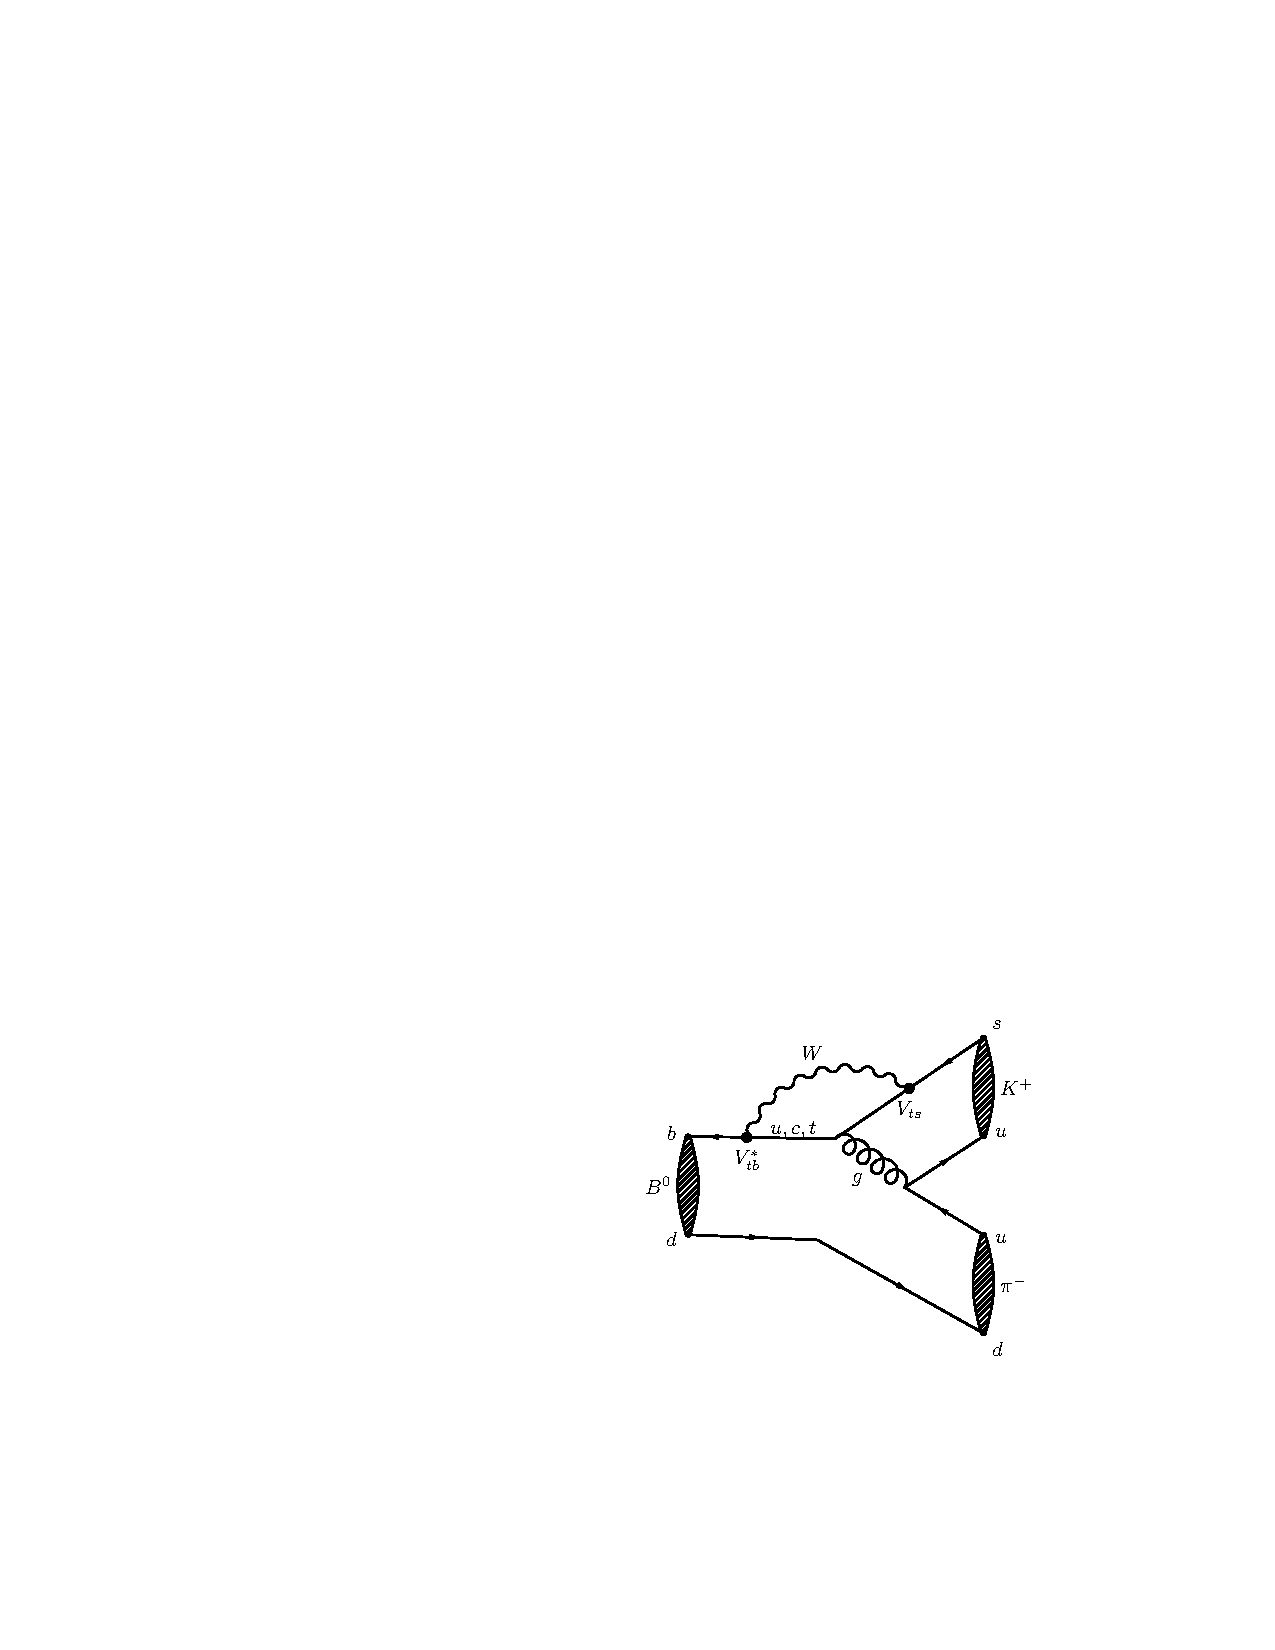
\includegraphics[width=0.4\textwidth]{problemsheets/fig/b_kpi_penguin.pdf}
\end{center}
\item The tree-level diagram has a strong phase $\delta_t$ related to the formation of final state hadrons, which is common for the $B^0$ and $\bar{B}^0$ decays. Similarly the loop-level diagram has a strong phase $\delta_l$. Show that
\[|\mathcal{A}_{B^0}|^2-|\mathcal{A}_{\bar{B}^0}|^2=2a_{t}a_{l}sin(\phi_t-\phi_l)sin(\delta_t-\delta_l)\]
where the magnitude of the tree and loop level amplitudes are $a_t$, $a_l$ respectively and the weak phase of the $B^0$ tree and loop diagrams are written as $\phi_t$ and $\phi_l$ respectively
\end{enumerate}

\NewQuestion{Basic Kinematics and detector design (exam style)}
An experiment is based at an $e^+e^-$ collider with a Centre of Mass energy of 91~GeV. The experiment aims at measuring the rate at which $Z^0$'s decay to a $b$ and a $\bar{b}$ quark.
\begin{enumerate}
\item Draw the Feynman diagram of this process
\item What are the energies and momenta of the out-coming $b$ and $\bar{b}$ quarks?
\item Will the experiment detect the $b$ and $\bar{b}$ quarks directly? If not explain why
\item By assuming that the hadrons containing a $b$ or $\bar{b}$ quark have a proper lifetime of 1~ps and that they carry on average 80\% of the momentum of the $b$ quarks, what is the average distance these hadrons will fly before decaying?
\item Discuss what type of a particle detector component is required in order to make sure experimentalists can separate $Z^0\to b\bar{b}$ decays over $Z^0$ decays to light quarks ($u$,$d$,$s$)
\item What type of detector components are required in order to measure the energies of particles produced from the $Z^0\to b\bar{b}$ process?
\end{enumerate}


%\NewQuestion{Cherenkov Detectors}